\documentclass[5p,authoryear]{elsarticle}
\makeatletter 
\def\ps@pprintTitle{%
 \let\@oddhead\@empty
 \let\@evenhead\@empty
 \let\@evenfoot\@oddfoot} % Supprimer le bas de page ELSEVIER
\makeatother
\usepackage[utf8]{inputenc} % En unicode
\usepackage[T1]{fontenc}
\usepackage[english]{babel}
\usepackage[babel=true]{csquotes} % permet de faire \enquote{a} (« a »)
\usepackage[fleqn]{amsmath} % pour certains signes mathématiques
\usepackage{amsthm} % Pour \begin{gather}
\usepackage{booktabs} % pour \toprule (un style de tableau)
\usepackage{multirow} % Pour colonnes multiples des tableaux
\usepackage{amssymb} % Pour \leqslant (<=, >=)
\usepackage{float}
\usepackage{hyperref} % 
\usepackage[english]{cleveref} 

% adding Code Blocking
\usepackage{listings}
\usepackage{color}

\definecolor{dkgreen}{rgb}{0,0.6,0}
\definecolor{gray}{rgb}{0.5,0.5,0.5}
\definecolor{mauve}{rgb}{0.58,0,0.82}

\lstset{frame=tb,
  language=Java,
  aboveskip=3mm,
  belowskip=3mm,
  showstringspaces=false,
  columns=flexible,
  basicstyle={\small\ttfamily},
  numbers=none,
  numberstyle=\tiny\color{gray},
  keywordstyle=\color{blue},
  commentstyle=\color{dkgreen},
  stringstyle=\color{mauve},
  breaklines=true,
  breakatwhitespace=true,
  tabsize=3
}




%\bibliographystyle{elsarticle-num}
\bibliographystyle{elsarticle-harv}

\usepackage{fancyhdr}
\pagestyle{fancy}
\lhead{MSDS 458 - SEC 56}
\rhead{Lee, J.}

\begin{document}


\begin{frontmatter}

\title{Focused Web Crawler: \\NBA Team Specific News Articles}
\author{Jason Lee}
\address{Northwestern University, SPS \\Natural Language Processing \\2020SP MSDS 453-56}


\begin{abstract}

Information is power in the sports betting industry. When teams' news hits the web, betting syndicates need to be able to react with speed before market prices adjust. A web scraper, or spider, can crawl the internet collecting relevant information. The goal of this project is to develop a spider utilizing the Scrapy and Selenium packages in Python to collect National Basketball Association (NBA) team specific news. The spider will crawl from page to page scraping, parsing, and saving the relevant articles.

\end{abstract}



\begin{keyword}
Natural Language Processing (NLP) \sep NBA \sep Sports Betting \sep Web Scraping \sep Python \end{keyword}

\end{frontmatter}



%\linenumbers
\section{Introduction}\label{introduction}

The sports betting markets are presumed to be efficient markets by the time the closing price on each game is locked in \citep{market}. Fortunately for professional sports bettors, there is a difference between the opening line and the closing line for each game where there is opportunity to exploit inefficiencies for financial gain. Many of these lines move when new information about a team is released to the public. There is a delay between when critical news comes out and when sportsbooks adjust their lines. Professional sports bettors are able to use the lag in the shifting lines advantageously by reacting the fastest with new information. Professional sports bettors are able to do this by utilizing automated bots or web crawlers, also known as Spiders. These Spiders scour the internet searching for any relevant sporting news that can add value to the sports bettors. 


This project focuses on building one of these Spiders to crawl the internet searching for news articles relating to any National Basketball Association (NBA) team. The spider will then parse and save important information that can then be used to inform sports betting decisions. This project will be sponsored by A.I. Sports and the final product will be utilized by their company to consult with various betting syndicates \citep{aisports}.


This project will also be the starting point for future natural language processing (NLP) projects. The focused web crawlers will collect hundreds of news articles combined together creating a complete corpus. The corpus will be broken down using document vectorization methods to understand relationships between each article in the corpus. There will be document classification models built on the corpus, as well as unsupervised machine learning techniques and multivariate analysis to better understand themes and sentiments of each article. Another future project will consist of developing a document summarization algorithm that can quickly generate accurate summarized outputs for each article. 


There are several desired outcomes from this first project: 1 – Create a fully functional and focused Python based web crawler. 2 – Understand how to inspect websites to extract the right information. 3 – Create a complete corpus of NBA team news articles for future Natural Language Processing (NLP) projects. 



\section{Literature Review} \label{lit_rev}


The process of extracting and storing information from the internet in an automated fashion is a highly valuable skill that requires a keen attention to detail. Writing flexible code that is able to handle potential errors is crucial for a successfully programmed focused web crawler. Three researches with ties to IBM dedicated time formulating a list of eight pivotal steps when creating a focused web crawler \citep{focused}:

\begin{enumerate}
 \item Canonical Taxonomy Creation
 \item Example Collection
 \item Taxonomy Selection and Refinement
 \item Interactive Exploration 
 \item Classifier Training
 \item Resource Discovery 
 \item Distiller Development
 \item Evaluation and Feedback
\end{enumerate} \\


The beginning step is obvious, create a topic for the focused web crawler to search. The next step is to collect example websites containing information about the chosen topic. During the example collection process, the following step naturally takes shape as the topic becomes refined. Certain websites and links may be marked as "good" or "bad" during both the example collection and refinement steps \citep{focused}. 

Once the topic has been narrowed down, an interactive exploration of the websites begins. A key feature to any focused web crawler is a specific starting (or multiple starting points) and a designated stopping point \citep{crawl}. A focused web crawler must have a purpose, which requires the user to perform preparatory work by traversing the internet to find key domains with relevant information. 

Once these starting domains are selected, the Spiders will be able crawl through each link, moving from webpage to webpage. However, there are many links on relevant websites that might lead to irrelevant material or advertisements. If the web crawler is left on its own, it may end up falling down the endless black hole that is the internet.

There are many ways to control the web crawler by setting program hyperparameters. The Spiders can be given strict instruction to remain only on specific domains. The Spiders can also be stopped after a predetermined number of pages deep it moves. Another program hyperparameter is the total number of pages to download, forcing the web crawler to immediately stop when it reaches the maximum limit \citep{crawl}. 

Step 5 in the IBM researchers list, training the classifier, helps the web crawler remain on a focused path. A classifier is a model that determines how relevant a particular website is to the chosen topic \citep{focused}. The classifier will allow for advanced filtering through websites that would not be feasible manually on larger projects. The classifier training takes into account the websites and domains manually marked as "good" and "bad" from the previous steps. 

\begin{figure}[!h] 
    \centering
	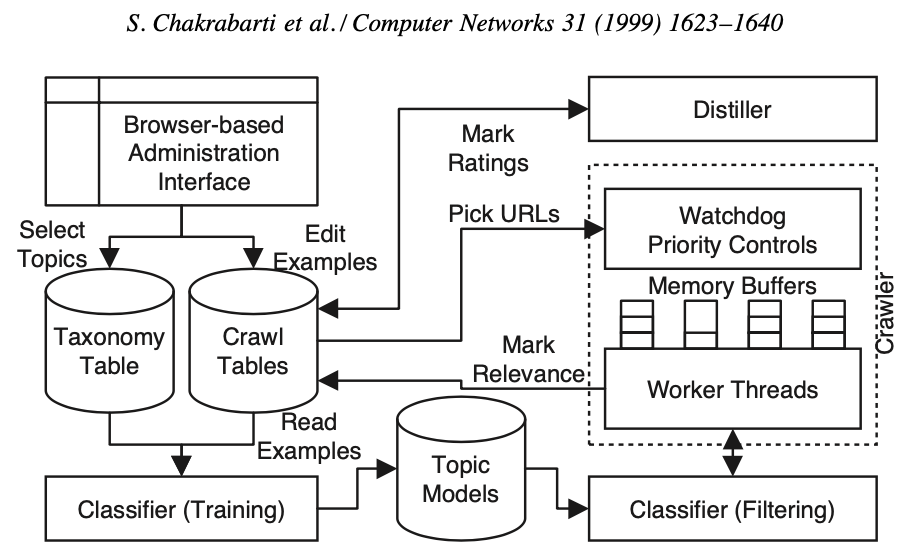
\includegraphics[width=3.4in]{figures/focused_webcrawler_diagram.png}
	\caption[]{Block diagram of the focused crawler showing how the web crawler, classifier, and distiller are integrated.} 
	\label{web_flow} 
\end{figure}

The final steps bring the entire project together. The user discovers the resources that were collected by the focused web crawler as it scrapes the internet. The user will be able to provide feedback that is cycled back into the classifier retraining and improving the outputs. A distillation algorithm can also be run after the focus web crawler has been working for some time. The distiller will be able to find key domains that are known as the authorities on the given topic. Figure \ref{web_flow} visually depicts the eight steps seamlessly flowing together in a diagram that was used by the IBM researchers, with the classifier, distiller, and crawler as the three focal components \citep{focused}.


\subsection{Scrapy}\label{Scrapy}

Scrapy is a Pyhonic program designed specifically for web crawling and scraping \citep{scrapy}. Figure \ref{Scrapy_Framework} shows how Scrapy behaves, which has some similarities to the IBM researchers' Framework in Figure \ref{web_flow}. The Spiders send the initial request to the Scrapy Engine, where the Engine checks the scheduler before dispatching the Spiders to the internet. The Spiders send their requests to the internet and receive a response. 

The Spiders have predetermined items they are sent to collect. The Spiders will internally scan the response sending each item it finds through the Item Pipeline where it is stored. The Item Pipeline is where the items can be parsed, transformed, and formatted before they are saved to the desired database or file.

\begin{figure}[!htb] \centering
	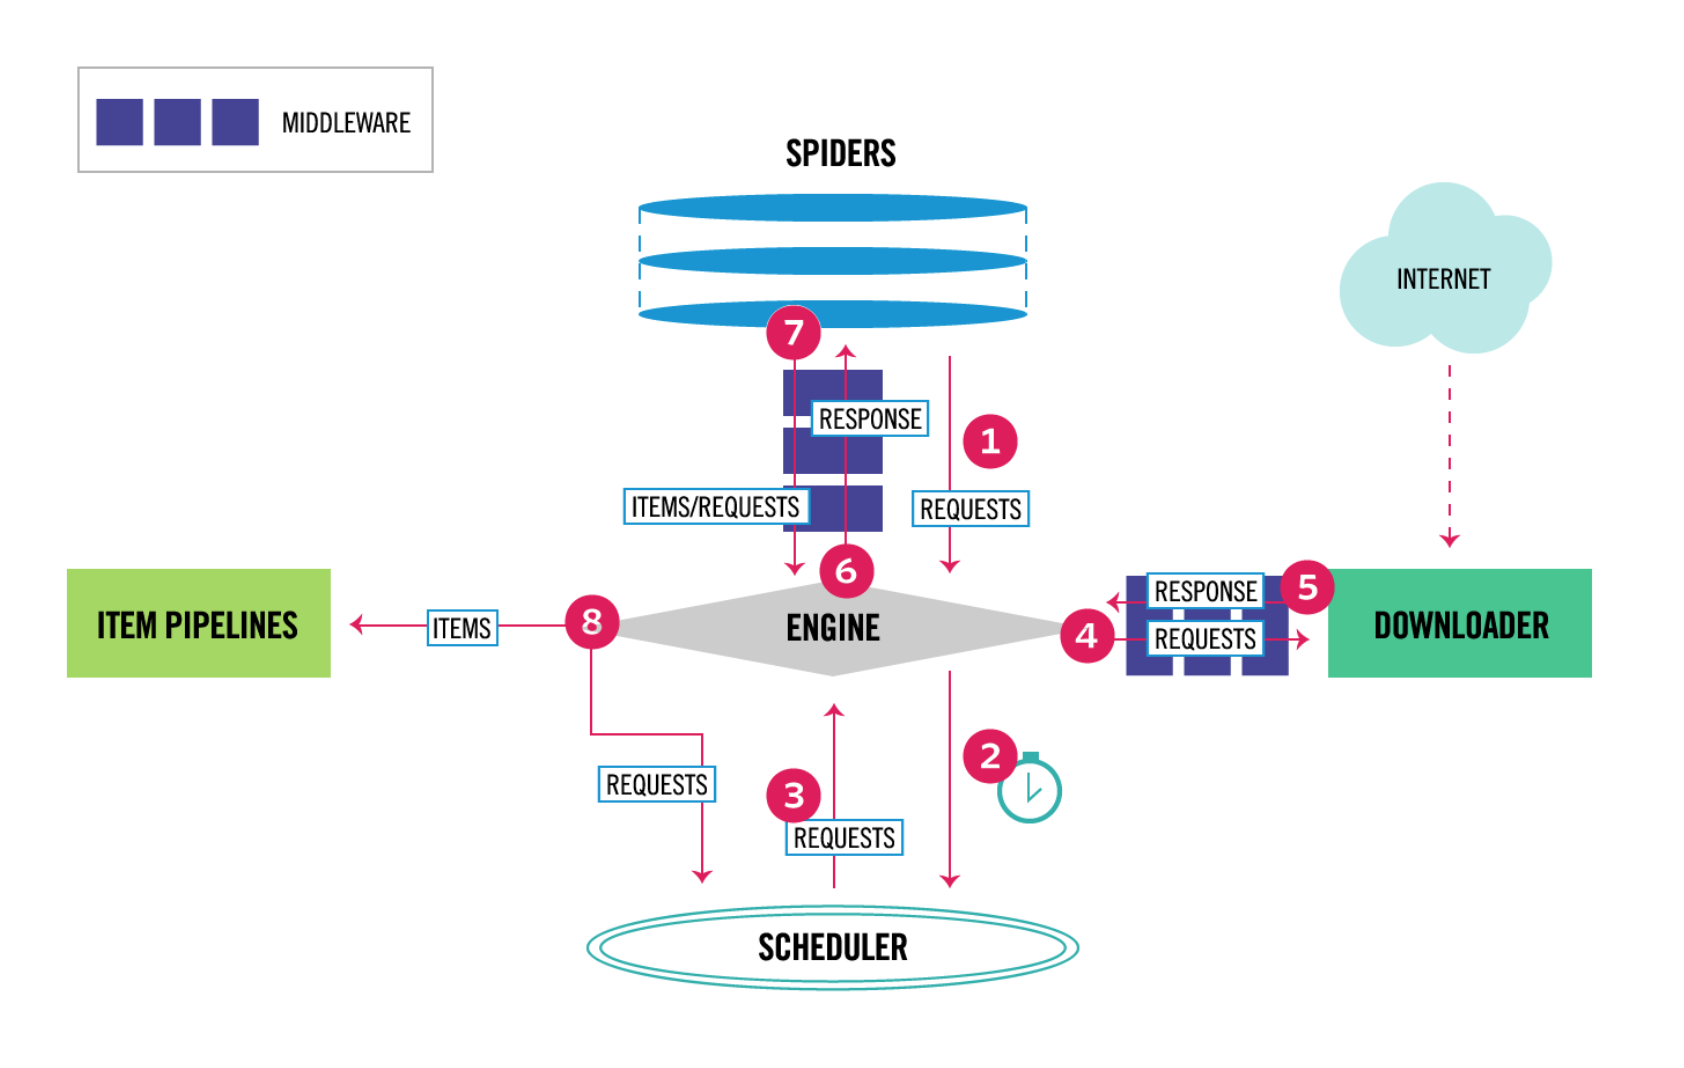
\includegraphics[width=3.7in]{figures/Scrapy_Framework.png}
	\caption[]{Illustration of the Scrapy Framework} 
	\label{Scrapy_Framework} 
\end{figure}

\subsection{Selenium}\label{Selenium}

Many newer websites are written with JavaScript and Angular applications embedded into the HTML code to allow the page to operate in a smooth, reactive fashion \citep{angular}. However, while the user experience is enhanced, these websites cause serious issues for most web crawlers as they try to extract the page contents. 

From the perspective of the Spiders, there are only empty containers where the contents should be because the webpage does not actually queried the server and load. Selenium is a tool that launches a WebDriver with a designated browser to allow the Spider to view a website the same way a user would view it. 

Figure \ref{Selenium_Framework} shows the Framework that Selenium operates within. There are many different types of browsers that can be used and the HTTP requests to the server and JavaScript code will run within Selenium. This allows the spiders to "click" buttons, scroll, and extract the information on these pages.


\begin{figure}[!htb] \centering
	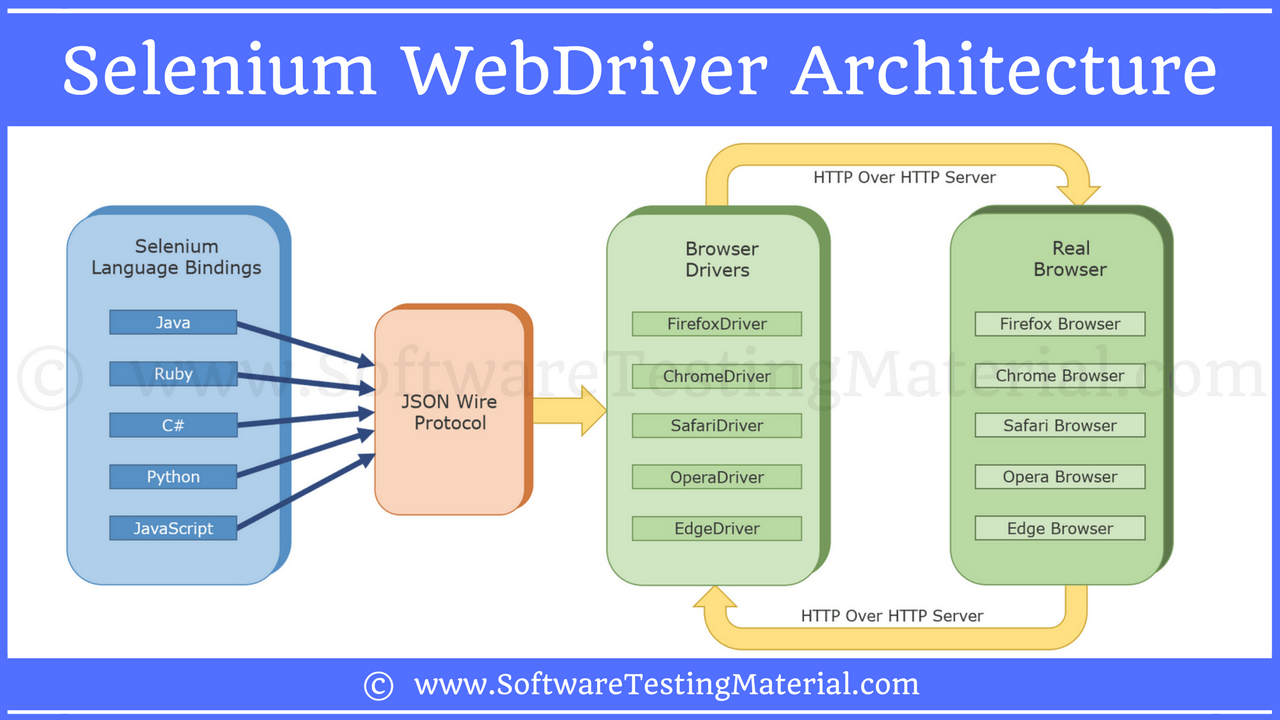
\includegraphics[width=3.4in]{figures/Selenium_Framework.png}
	\caption[]{Illustration of the Selenium Framework} 
	\label{Selenium_Framework} 
\end{figure}


\section{Methodology}\label{meth}


The methodology implemented during this project is as follows. 


\subsection{Topic Selection and Refinement}\label{chat}

The canonical topic chosen for this project is the National Basketball Association (NBA). More specifically, news articles discussing team match-ups, injuries, and general news that might give insight into how the team will perform in their upcoming games. 

Gathering relevant examples was an easy task, almost too easy. There are local beat writers, national news coverage, bloggers, and the occasional deep dive investigative reporting from media companies. 

Unfortunately, the main sports news companies, like ESPN, FOX Sports, Turner, Bleacher Report, etc., do not cover teams equally or fairly. There are 30 NBA teams and each team has dedicated team website on NBA.com. An assumption by using the official team specific websites is that each team's news will be biased towards their own team. This is an acceptable bias for this project because of the consistency across all of the teams.

The web crawlers will begin on each team's official NBA website and move from post to post scraping each article. 



\subsection{Interactive exploration of the web}\label{exploration}

\begin{figure}[!htb] \centering
	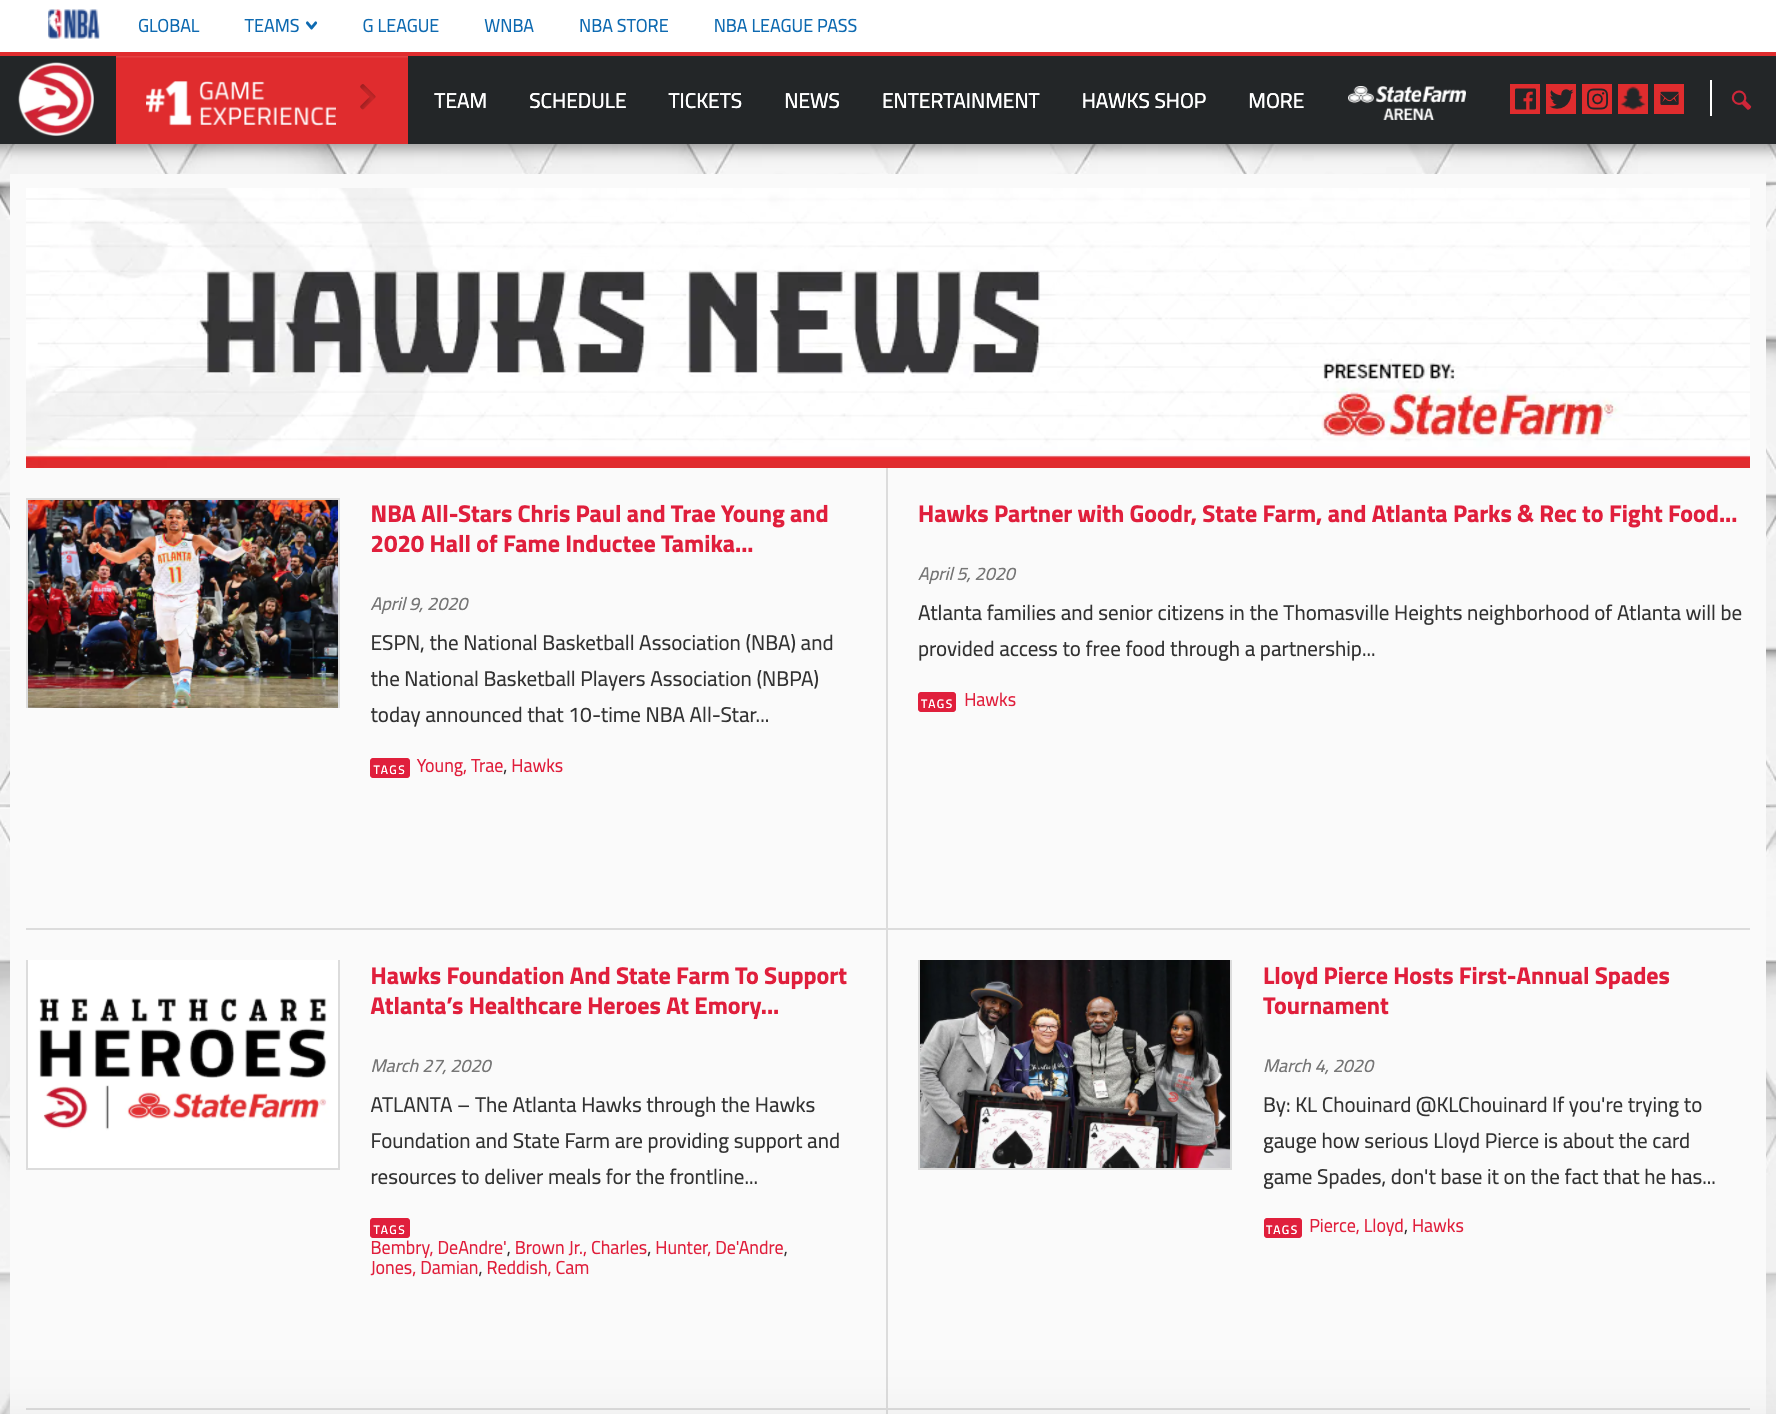
\includegraphics[width=3.4in]{figures/Hawks_News.png}
	\caption[]{Atlanta Hawks News homepage} 
	\label{hawks news} 
\end{figure}

This portion of the project was extremely tedious. There were many issues trying to program the web crawlers. The Atlanta Hawks are the first alphabetical team in the NBA making them the experimental guinea pig. Their web page is shown in Figure \ref{hawks news}. 

\begin{figure}[!htb] \centering
	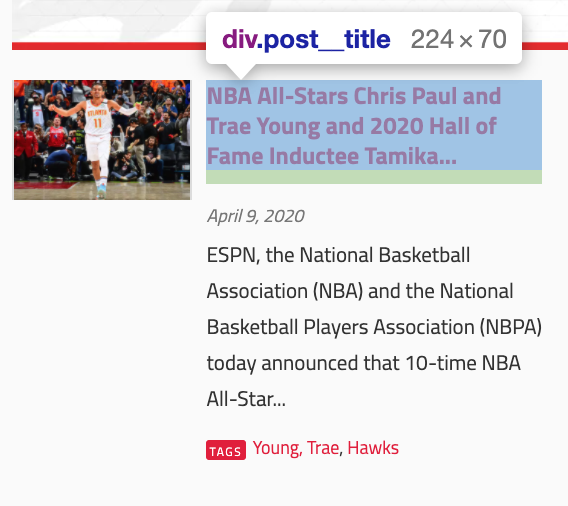
\includegraphics[width=3.0in]{figures/post_title.png}
	\caption[]{HTML Class = 'post\_\_title' showing where the web crawler can extract the information on the news article's title} 
	\label{Post Title} 
\end{figure}

The first step is to open the developer tools and inspect the raw HTML code searching for the XPATH or CSS class name, or id tag, for the section on the website that will be scraped. Figure \ref{Post Title} shows an example of the article's title class for the web crawler to find. Looking over the website's code and finding the class names, this appears to be a fairly simple and straightforward task for the focused web crawler to complete. 


\begin{figure}[!htb] \centering
	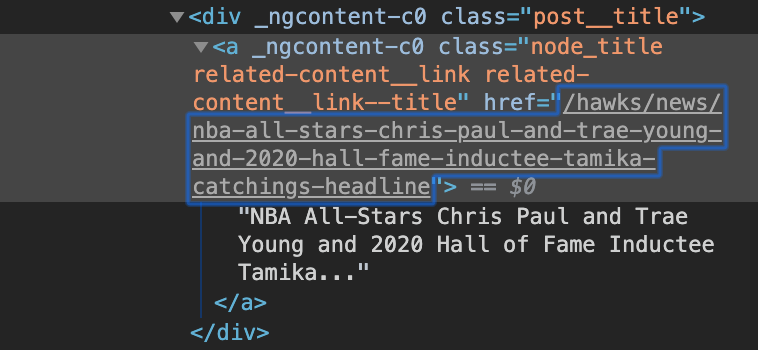
\includegraphics[width=3.0in]{figures/post_link.png}
	\caption[]{The HTML Hyperlink is contained within the 'post\_\_title' div allowing the spider to crawl to the actual new article's page to scrape the entire document} 
	\label{Post Link} 
\end{figure}



However, this did not work at all. In Figure \ref{Post Link}, there is a tag "\_ngcontent" meaning that this information is contained inside an Angular JavaScript application. This issue and coming up with a workable solution dominated the majority of the allotted time to complete this project. Eventually, the Spiders were able to collect the necessary information by using both Selenium and Scrapy together.


\section{Computational Experiment}

The entire Python code for this project's focused web crawler program will be attached to this paper, or can be reproduced by cloning the project's \href{https://github.com/papagorgio23/NBA_News_Spiders}{Github Repository} at this url:\\

\href{https://github.com/papagorgio23/NBA_News_Spiders}{github.com/papagorgio23/NBA\_News\_Spiders}\\ 

To run the program, simply type the following line of code into the command line from the "NBA\_News\_Spiders" project home directory: 

\begin{lstlisting}
    cd NBA_News
    python release_spiders.py
\end{lstlisting} 

This script will unleash the spiders onto hundreds of NBA news articles where they can scrape relevant information. This program will output the articles in an itemized JSON line file, where each line in the file contains a single news article and key associated details. Those details include the team, url, date, tags, and the article.


\subsection{Release Spiders Python Script}\label{release}

The "release\_spiders.py" file is an adapted version of the "run-articles-spider.py" file from the "WebFocusedCrawlWorkV001" directory \citep{sample-code}. The file begins by creating a folder called "nba\_articles" where the downloaded html web pages will be saved by the Spiders as they crawl from site to site. 

The structure of the directory is then outputted to the terminal ensuring that everything is in order before the spiders are released into the wild. The final lines of code call on Scrapy to launch the focused web crawlers and save the items in a JSON line formatted file. 



\subsection{Scrapy with Selenium}


The workhorse script for this focused web crawler program is found in the spiders folder with the title "articles\_spider.py". The Spider named "ArticlesSpider" is created with instructions to perform two sequential tasks. 

Typically, when a Scrapy Spider is released, it is given a list of URLs to start their crawl. What is unique about this particular Spider is that the starting URLs is a function call instead of a list of URLs. This function initializes a Selenium webdriver with a headless Chrome browser. Through Selenium, the Spider loops through a list of each team's news website clicking the "load more" button eight times to expand the number of news articles displayed on the web page to a maximum 96 articles. 

Once the articles are all loaded into the browser, the Spider collects the URLs for every single news article. This complete list with hundreds of URLs from every team is then passed back to the Scrapy Spider and the Selenium browser closes. The Scrapy Spiders will then use this returned list of URLs as starting points to crawl each article, parsing and storing the required information. 





\subsubsection{Items}

The Scrapy items Python script is used for two purposes. First, the items that the Spiders are searching for are defined. The Spiders will collect six important pieces of information from every article:

 \begin{enumerate}
 \item team  = The name of the NBA team
 \item url = The URL where the article is found
 \item tags = The topic tags for the article
 \item title = The title of the article
 \item date = The date the article was posted
 \item article = The complete article
\end{enumerate} \\

The second purpose of the items script is to preprocess, or clean, some of the fields before they are stored. The raw date field would return a character string similar to this: 

"Posted on: Mar 14, 2020" 

This is not a workable format for a computer to understand. A custom function is written to trim "Posted on: " from the string and then "Mar 14, 2020" is converted into a Python Datetime field. The result of this function is then stored as the date item for each article. 

The other field that requires preprocessing is the article field. The articles are comprised of many elements, such as links, special characters, and lingering HTML tags. The Spiders also capture leading and trailing text that is not actually apart of the story. 

The first step cleaning this field comes by utilizing the remove\_tags function from the w3lib.html library. The trailing text always beings with "Copyright", making it a convenient word to split at to remove the irrelevant text. The leading text is consistent across the articles making it simple to remove as well. Finally, paragraph breaks and excess spaces are trimmed and the cleaned article string can be stored. All of these steps can found in the "items.py" script in the NBA\_Scrapy folder.  



\section{Results}

The Scrapy program logs are shown in Figure \ref{Scrapy Results}. The Scrapy spiders crawled 771 links, extracting 768 itemized articles. Unfortunately, there were consistency issues between many of the NBA team's homepages. There were seven NBA teams that returned zero news articles, resulting in a total of 23 NBA teams represented in our corpus. While this is not optimal, it is an acceptable corpus size to meet the requirements. 

\begin{figure}[!htb] \centering
	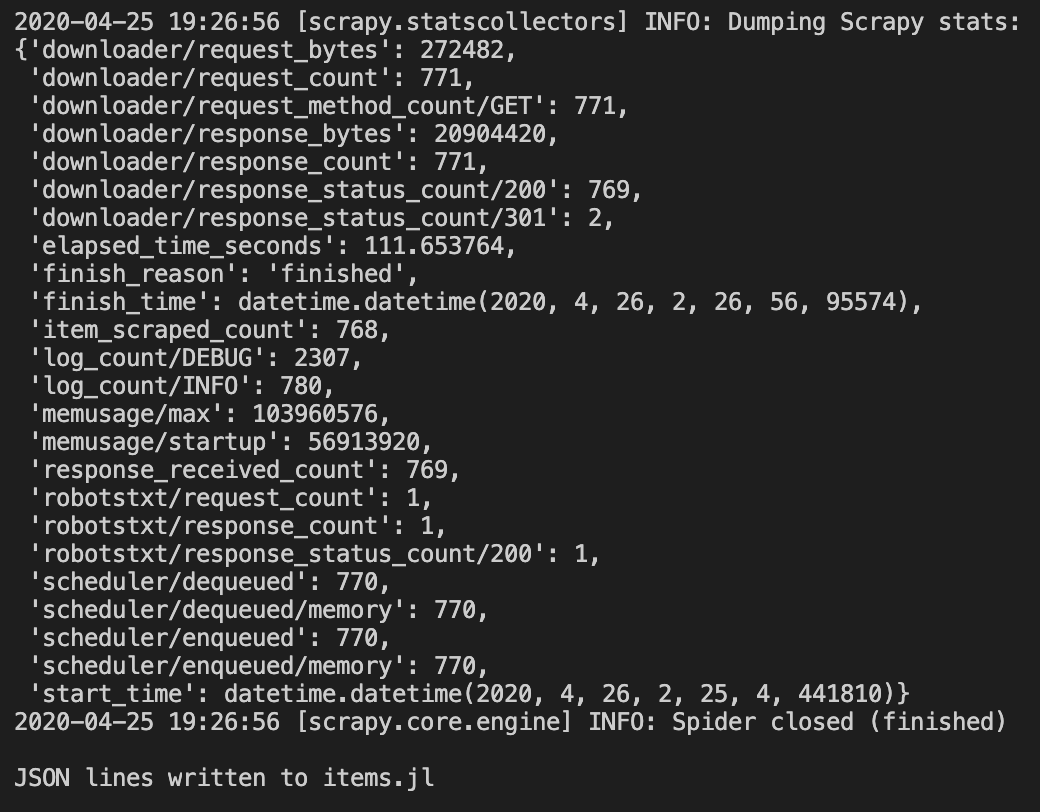
\includegraphics[width=3.0in]{figures/Scrapy_Results.png}
	\caption[]{Scrapy output logs from the focused web crawler program} 
	\label{Scrapy Results} 
\end{figure}

Roughly 23 minutes elapsed to completely run the focused web crawler program, with the Selenium portion absorbing a disproportionate amount of the time. Selenium takes up so much time because each time a spider lands on a team's homepage, there is a programmed delay to allow the Angular application and JavaScript portions of the page to load. The spider then tries to click eight buttons, waiting a few seconds in between each click for the news articles to populate before the contents can be extracted. 

Once the Selenium portion finished collecting the 771 usable links to news articles, the Scrapy spiders were able to scrape each article in under two minutes. The Scrapy Spiders saved the itemized JSON file, as well as the full HTML webpage for all 768 articles.


\section{Discussion and Conclusions}

Potential future work to improve the performance of this focused web crawler and scraper would include adding additional error handling steps to hopefully collect news articles from all 30 teams. There were several NBA teams who have not updated their websites, meaning that they do not follow the same standard design template. Because of the time constraints for this project, there was not enough time to manually investigate the websites of each of the teams that through an error. Fixing this code will allow the spiders to scrape hundreds of additional articles.

Another slight programming issue came trying to incorporate the Selenium driver within the Scrapy framework. The initial plan was to use Selenium on each team's website by placing a Selenium driver within the "start\_requests" function in the Spider's Class. However, this generated issues managing the number of drivers opened and transitioning the request from using Selenium on the starting JavaScript team page to using the standard Scrapy request and response on the static article page. The ideal plan would utilize the middlewares.py Scrapy functionality by adding Selenium into the "process\_request" function (Step 4 in the diagram in Figure \ref{Scrapy_Framework}). Ultimately, the attempts to implement this failed under the given time frame but future work should make this adjustment. 

In conclusion, this project was able to accomplish each of the goals originally laid out. A fully automated and narrowly focused web crawler was built in Python utilizing both Scrapy and Selenium that A.I. Sports will be able to use in the future. There has been a deeper understanding of website structure and tools need to extract the right information over the life cycle of the project. And finally, an organized corpus of NBA team news articles has been created for future natural language processing (NLP) projects.


\clearpage

\bibliography{bibliographie.bib}

\bibliographystyle{newapa}

\end{document}